\section{Use Case}

This section compares an implementation of a simplified Pac-Man game (Figure~\ref{fig:pacman}) in Haskell
with \dsl{}\footnote{\url{https://github.com/rubenpieters/PaSe-hs/tree/master/PaSe-examples/Pacman}} and TypeScript with GSAP\footnote{\url{https://github.com/rubenpieters/pacman-ts}} both quantitatively and qualitatively. The
quantitative evaluation compares development time and lines
of code. The qualitative one compares different aspects of the 
libraries.

\begin{figure}[h]{\textwidth}
\centering
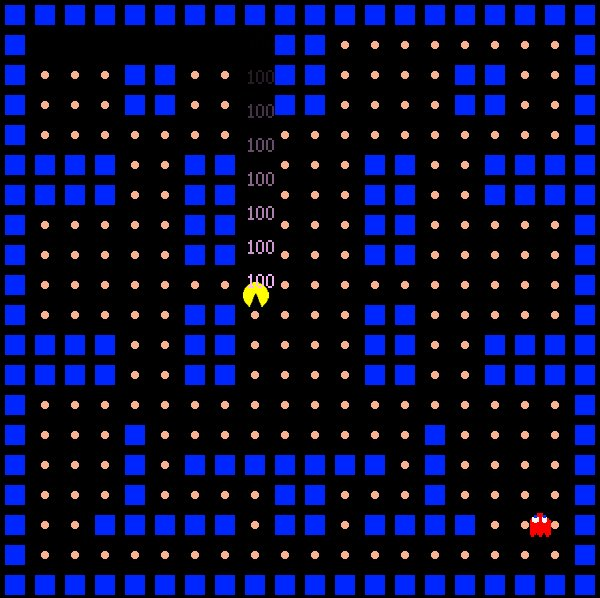
\includegraphics[width=.3\textwidth]{pictures/pacman}
\caption{Screenshot of the Pac-Man application.}
\label{fig:pacman}
\end{figure}

\subsection{Quantitative Evaluation}

This section compares the PaSe and GSAP implementations on
quantitative criteria. We consider the development time and lines of code for
each module.

\begin{itemize}
\item \textbf{Development Time} The Haskell application was developed in
$\sim$1.5 working days, while the TypeScript application took $\sim$1 working
day. We consider this approximately the same development time as the Haskell application
was developed first, and thus contains design work shared by both
applications. The developer is proficient in both languages.
\item \textbf{Lines of Code (LOC)} Table~\ref{tbl:loc} contains the LOC data
(including whitespace) for both applications. Their total LOCs are roughly the same. However, the Haskell
code implements its own functionality for sprites and
textures while we used the existing
\texttt{Sprite} class of the \texttt{PixiJS} library in TypeScript.
\item \textbf{Relative LOC} Table~\ref{tbl:loc} also contains the relative
LOCs. The GSAP animation definitions (AnimDefs) are slightly bigger because
we had to embed effects in the animations due to differences
in the used graphics library, and because of TypeScript's relative verbosity.
Using the timeline feature of GSAP, the code for
simple animations is comparable to PaSe. However for more complex animations
and those requiring embedded effects, there are some differences which we
discuss in more detail in the qualitative evaluation.
\end{itemize}

\begin{table}[t!]
\caption{Lines of code comparison (including whitespace)}
\centering
\label{tbl:loc}
\begin{center}
\begin{tabular}{l@{\hskip 0.5cm}rr@{\hskip 0.2cm}rr}
 \textbf{Module} & \textbf{Haskell/PaSe (LOC)} & \textbf{\%} & \textbf{TypeScript/GSAP (LOC)} & \textbf{\%} \\
 \hline
 AnimDefs & 127 & 21\% & 197 & 32\% \\ 
 Anims & 43 & 7\% & 39 & 6\% \\  
 Field & 48 & 8\% & 77 & 12\% \\  
 Game & 130 & 21\% & 113 & 18\% \\  
 Main & 36 & 6\% & 23 & 4\% \\  
 Sprite & 45 & 7\% & / & / \\  
 Textures & 34 & 6\% & 13 & 2\% \\  
 Types & 10 & 2\% & 3 & 0\% \\  
 View & 139 & 23\% & 158 & 25\% \\
 \emph{Total} & \emph{612} & \emph{100\%} & \emph{623} & \emph{100\%}
\end{tabular}
\end{center}
\end{table}

\subsection{Qualitative Evaluation}

This section compares PaSe and GSAP on five qualitative criteria.

\begin{itemize}
\item \textbf{Eco-system} Animations are not created in isolation; they need to
be coupled to a graphical backend to display them on the screen.  GSAP's maturity
makes it a clear winner here. It 
is well integrated with the browser and supports a rich set of features
such as a variety of plugins, compatibility across browsers and support for
animating a large range of DOM elements. Yet, for Pac-Man we only needed
lenses for our own user-defined state.
\item \textbf{Workflow} It is important that animations can
be specified easily and concisely. Creating pure animations, without
any embedded effects, are equally convenient in GSAP and in PaSe. However, more
complex interactions with effects and control flow are simpler in PaSe. We
saw this in the Pac-Man use case when implementing particle animations.
A particle animation is an animation that creates an object, animates it
and then destroys it again. We
implemented a general wrapper for such animations which takes as input a
function \hs{Int -> Animation}, where the \hs{Int} is the unique particle
identifier, and a creation and deletion function for the particle. In the GSAP
library we have to add the function to the timeline as a callback, which
means its duration is considered to be \hs{0}. This is problematic
because the deletion of
the particle should occur after its animation. This means that we are
forced to manually calculate and provide the duration for the particle
animation.
\item \textbf{Performance} Both libraries perform 
equally acceptable on Pac-Man: no visible glitches or lag at 60
frames per second (FPS) on an Intel core i7-6600U at 2.60 GHz with 8GB memory. We have also implemented a benchmark similar to GSAP's
speed test\footnote{\url{https://greensock.com/js/speed.html}}, which tests a large parallel animations. GSAP is
slightly more optimized currently as it handles 500 parallel animations at 60 FPS instead of \dsl{}'s 400.
This could be remedied by further performance improvements of \dsl{},
like fusing multiple parallel animations or improving the \hs{Animation} data structure, which are future work.
\item \textbf{Extensibility \& Inspectability} Extensibility and inspectability
are key features of PaSe. Both were useful for Pac-Man. Inspectability allowed 
extracting all used textures in the animations to
automate their loading. Extensibility enabled the definition of the 
particle effect mentioned earlier. We
created a new \hs{WithParticle} type class and implemented both an
\hs{Animation} instance and a \hs{Const} instance for the texture inspection.
GSAP does not support inspectability, and thus we did not
implement the automatic loading of textures. The particle animation function
was implemented with callbacks and implicit side-effects, which TypeScript allows anywhere.
\end{itemize}
